\begin{figure}[p]
\centering
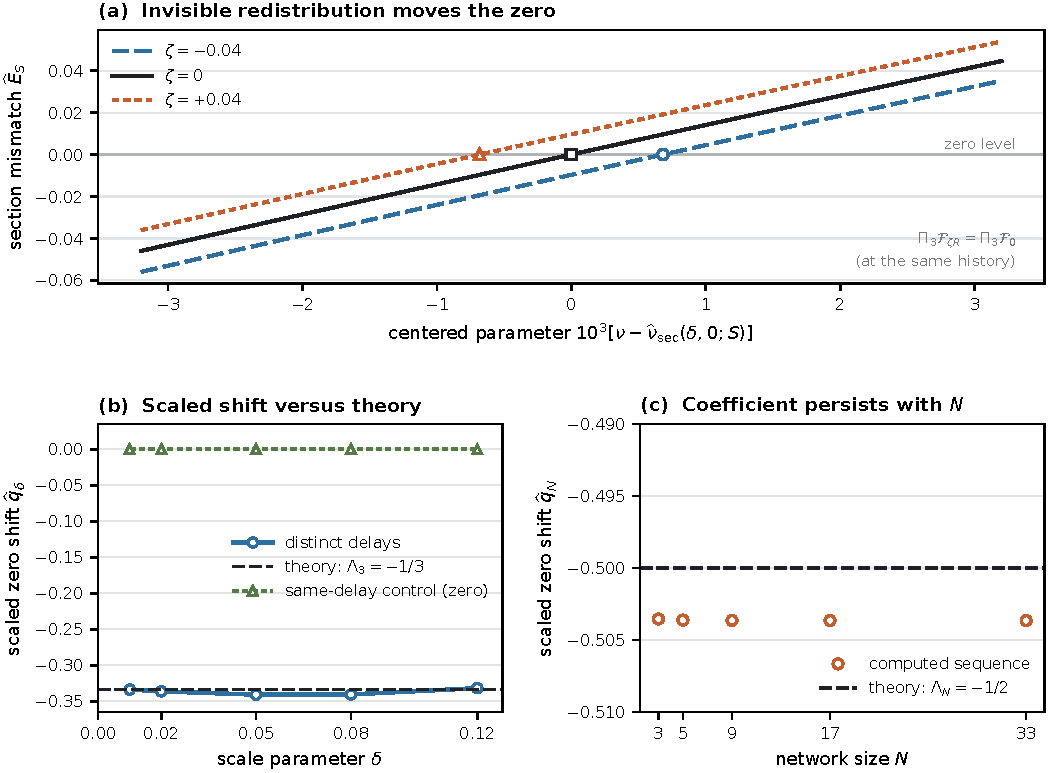
\includegraphics[width=\textwidth]{figures/three-node-finite-section.pdf}
\caption{Prescribed-history section diagnostics for the local Fredholm
coefficient, with parameters from \cref{eq:numerical-section-quotient} and
its preceding paragraph.  \textbf{(a)} The marked zeros of
\(\widehat E_S=Y(S)-X(S)^2+1/2\) shift under opposite perturbations of the two
delay layers, while the projected vector field is unchanged at each fixed
history; \((\delta,S)=(0.05,3)\).
\textbf{(b)} The computed quotient is compared with \(\Lambda_3=-1/3\) along
\((\delta,S)=(0.12,2.5),(0.08,2.75),(0.05,3),(0.02,3.5),(0.01,4)\).
Combining the perturbation layers at one delay makes their contribution
cancel exactly (green triangles).
\textbf{(c)} The growing family at \(N=3,5,9,17,33\) has computed quotients
close to its common coefficient \(\Lambda_N=-1/2\).  Symbols and curves are
numerical; dashed reference coefficients and the cancellation identity are
analytic.  This calculation is not \(D_N^{\rm fin}\) and does not compute a
heteroclinic connection or a maximal canard.}
\label{fig:three-node-finite-section}
\end{figure}
